\section*{SMP and Gale Shapley}
\begin{itemize} %[itemsep=0ex,topsep=-2ex]
    \item instability: say $(m, w')$ is instable if 
    \begin{itemize}[leftmargin = 1em]
        \item $m$ prefers $w'$ more than his current $w$, and
        \item $w'$ prefers $m$ more than her current partner $m'$
    \end{itemize}
    \item note: the set S returned by GS is unique, even if 
    there's more than one perfect pairing
    \item runtime: $\Theta(n^2)$
\end{itemize}
    % insert Gale Shapley Code
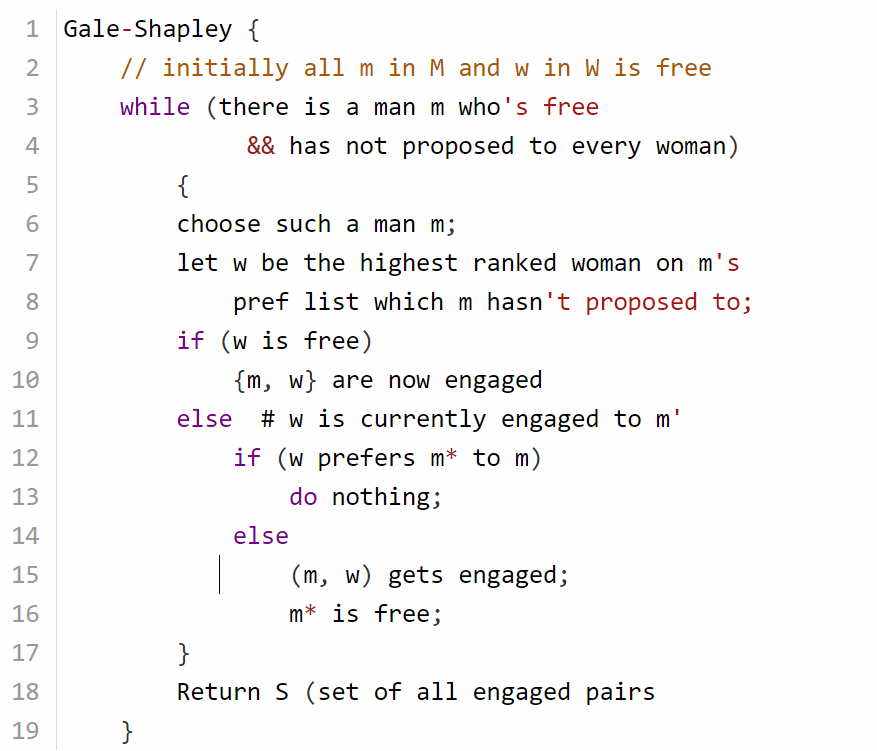
\includegraphics[scale = 0.61]{pictures/gale-shapley code.png}

    % \begin{verbatim}
    % Gale-Shapley {
    % // initially all m in M and w in W is free
    % while (there is a man m who's free 
    %          && has not proposed to every woman) 
    %     {     
    %     choose such a man m;
    %     let w be the highest ranked woman on m's 
    %         pref list which m hasn't proposed to;
    %     if (w is free)
    %         {m, w} are now engaged
    %     else  # w is currently engaged to m'
    %         if (w prefers m* to m) 
    %             do nothing;
    %         else 
    %             (m, w) gets engaged;
    %             m* is free;
    %     }
    %     Return S (set of all engaged pairs
    % }
    % \end{verbatim}
